\documentclass[
    12pt, % Schriftgröße
    ngerman, % für Umlaute, Silbentrennung etc.
    a4paper, % Papierformat
    oneside, % einseitiges Dokument
    headings=big, % Größe der Überschriften verkleinern
    nolistof=totoc, % Verzeichnisse nicht im Inhaltsverzeichnis aufführen, eigene Einstellung
    bibliography=totoc, % Literaturverzeichnis im Inhaltsverzeichnis aufführen
    index=totoc, % Index im Inhaltsverzeichnis aufführen
    captions=tableheading, % Beschriftung von Tabellen unterhalb ausgeben
    final % Status des Dokuments (final/draft)
    %toc=chapterentrywithdots %Inhaltsverzeichnis mit Punkten
    sectionentrydots=true   %Sectioneinträge in IHV mit Punkten versehen
]{scrreprt}
%scrreprt -> Basis der Befehle: Koma Script siehe 500+ Seiten Anleitung



%Dies sind die im Main verwendeten Pakete. Genauere Optionen und Einstellungen finden sich unter der cTan des jeweiligen Pakets. (https://ctan.org/)


%Allgemeine Pakete
\usepackage[utf8]{inputenc} 
\usepackage[ngerman]{babel}                         %Landessprache Deutsch
\usepackage[T1]{fontenc}                            %Schriftformatierung

% Graphik- und Tabellenpakete
\usepackage[pdftex]{graphicx}                      %Implementierung 
\usepackage{pdfpages}
\graphicspath{{img/} }                              % Ordner für die verwendeten Bilder
\usepackage{subfig}                                 % Paket für mehrere Graphiken nebeneinander
%\usepackage{tabularx}                               % Tabellenpaket 1
%\usepackage{tabulary}                               % Tabellenpaket 2
\usepackage{array}


%Tabellen für Formeln und Gleichungen
\usepackage{amsmath}


%Schriftdarstellung und Textoptimierung 
\usepackage{mathptmx}               % Schrifteinstellung für Times New Roman
\usepackage{microtype}              % Blocksatzbildung
\usepackage{color}                  % Möglichkeit zum Verwenden von Farben
\usepackage{lmodern}                % bessere Fonts
\usepackage{relsize}                % Schriftgröße relativ festlegen
\usepackage{blindtext}              %Packet Blindtext zum Einfügen von sinnlosen Text

% Pakete für Blattgeometrie und Seitenabstände - genaue Einstellungen unter einstellungen.tex
\usepackage{geometry}               %zunächst auf Standardeinstellungen belassen...
\usepackage{setspace}               %Paket für vertikale und horizontale Abstände  


%Verzeichnispakete 
\usepackage[automark]{scrlayer-scrpage}             % Paket für Kopf und Fußzeile
\usepackage[printonlyused,withpage]{acronym}        % Abkürzungsverzeichnis
\usepackage{chngcntr}                               % Abbildungsverzeichnis
\usepackage[final]{listofsymbols}                   % Symbolverzeichnis
\usepackage{eurosym}                                % Europäsche Symbole
\usepackage{textcomp}                               % Weitere Symbole

\usepackage{float}                                  %Formelverzeichnispakete
\usepackage{remreset}                               %Formelnummerierung 

%Literaturverzeichnispakete und Zitierstileinstellung 
\usepackage[citestyle=numeric-verb,backend=biber,style=numeric]{biblatex}
\usepackage[autostyle,german=guillemets,german=quotes]{csquotes}
\addbibresource{literaturverzeichnis.bib}


% Pakete für Hyperlinks (erst ganz am Ende aktivieren!!)
%\usepackage[colorlinks,pdfpagelabels,pdfstartview = FitH,bookmarksopen = true,bookmarksnumbered = true,linkcolor = black,plainpages = true,hypertexnames = false,citecolor = black] {hyperref} %Erstellen von Hyperlinks
%\usepackage[figure]{hypcap}                        %Hyperlinks für Abbildungen


\usepackage{etoolbox}
%
%
% Dies sind die vor Grundeinstellungen für das Dokument. Hier werden Verzeichnisse umbenannt, Seitenabstände, Blattgeometrien, Kopf/Fußzeilen eingerichtet. 



%Schriftarten von Überschriften und Inhaltsverzeichniseinträgen einstellen:
\renewcommand{\rmdefault}{ptm}
\renewcommand{\sfdefault}{phv}
\renewcommand\familydefault{\rmdefault}
\addtokomafont{chapter}{\rmfamily\mdseries\Large \hspace*{-0.2cm}\vspace{-10pt}}
\addtokomafont{section}{\normalfont\large\rmfamily\mdseries\hspace*{-0.2cm}\vspace{-10pt}}
\addtokomafont{subsection}{\normalfont\large\rmfamily\mdseries\hspace*{-0.2cm}\vspace{-10pt}}
\addtokomafont{chapterentry}{\rmfamily\mdseries\large \hspace{0pt}\vspace{-0pt}}
\addtokomafont{part}{\rmfamily\mdseries\Large \hspace*{-0.2cm}\vspace{-10pt}}
\addtokomafont{partentry}{\vspace{-30pt}\rmfamily\mdseries\large \hspace{0pt}}

%Seitenabstände und Abstände zwischend den Kapiteln einstellen
\RedeclareSectionCommand[beforeskip=0pt,afterskip=\baselineskip,afterindent=false]{chapter}
\RedeclareSectionCommand[beforeskip=0pt,afterindent=false]{section}
\RedeclareSectionCommand[beforeskip=-10pt,afterskip=\baselineskip,afterindent=false]{subsection}

%Vertikalen Abstand zwischen Verzeichnissen und eigentlichem Text einfügen
\DeclareTOCStyleEntry[
  onstarthigherlevel=\addvspace{4em}
]{part}{chapter}
\DeclareTOCStyleEntry[
 onstarthigherlevel=\addvspace{3em}
]{section}{chapter}



%Umbenennen und Einstellen für das Tabellen und Abbildungsverzeichnsi
\KOMAoptions{listof=entryprefix}                                % Einstellung: Formulierung vor Verzeichniseintrag
\providecaptionname{ngerman}{\listoflofentryname}{Abbildung}    % "Abbildung" vor vor dem jeweiligen Vz. Eintrag
\providecaptionname{ngerman}{\listoflotentryname}{Tabelle}      % "Tabelle" vor vor dem jeweiligen Vz. Eintrag
\BeforeStartingTOC[lof]{\def\autodot{:}}                        % Doppelpunktsetzung Abbildungsverzeichnis
\BeforeStartingTOC[lot]{\def\autodot{:}}                        % Doppelpunktsetzung Tabellenverzeichnis
\counterwithout{figure}{chapter}                                % Verzeichniseinträge ohne Kapitelbezug
\counterwithout{table}{chapter}                                 

% Symbolverzeichniseinstellungen
\renewcommand{\symheadingname}{Symbolverzeichnis}               % Umbenennen
\setlength{\symwidth}{4cm}                                      % Abstand zwischen Symbol und Erklärung einstellen 


% Kopf- und Fußzeile der ersten Seiten (Paket scrlayer-scrpage)
\pagestyle{scrheadings}
\clearmainofpairofpagestyles{}  % alle Felder leeren
%\ihead{}\chead{}\chead{}
\cfoot{\pagemark}               % Seitenzahl unten mittig


%Absätze einstellen
\setlength{\parindent}{0cm}                     % Einrücken des Textes bei neuem Absatz
\setlength{\parskip}{0.5cm}                     % Vertikaler Abstand der Absätze
\doublespacing{}                                % Allgemeiner Zeilenabstand
%\setlength\abovecaptionskip{2cm}               % Abstand Tabellenunterschrift
%\mathsurround=3cm 

% Seitenränder für das Textdokument einstellen
\newgeometry{left=4cm, right=2cm, top=2cm}
\setlength{\headheight}{1.5cm}                  % Höhe Kopfzeile
\setlength{\voffset}{2.5cm}                     % Abstand Oberer Rand - Textfeld
\setlength{\topmargin}{-4.5cm}                  % Abstand Oberer Rand - Text oben
\setlength{\headsep}{0.5cm}                     % Abstand Kopfzeile - Text oben 
\setlength{\footskip}{2cm}                      % Abstand Fußzeile - Text unten
\setlength{\footheight}{1.5cm}                  % Höhe Fußzeile

%Abstand Gleitumgebungen zum Text
\setlength{\intextsep}{12pt}
\setlength{\textfloatsep}{12pt}


%\overfullrule=20pt

%Abstände Tabelle:
%\usepackage{caption}
%\captionsetup[table]{position=below,skip=2cm}
%\setlength{\abovecaptionskip}{2cm}             %Abstand Tabelle - nachfolgenden Text






\begin{document}

\pagenumbering{Roman}
\thispagestyle{empty}
\begin{tabular}{p{\textwidth}}
\centering{
\doublespacing{}
\large {Private Fachhochschule für Wirtschaft und Technik \\
Bachelor of Engineering\\
Ausbildungsbetrieb: DIL Engineering GmbH}\\
\par}

\vspace{1cm}

\begin{center}

\includegraphics[width=\textwidth]{img/PHWT-Logo.jpg}\\
\end{center}

\vspace{0.5cm}

\begin{center}
\large{Praxistransferbericht zum Thema:\\}
\end{center}

\begin{center}
\Large{Auslegung eines Druckbehälters nach Merkblatt AD2000}
\end{center}

\vspace{0cm}

\begin{center}
Beschreibung 1\\
\end{center} 

\vspace{0.2cm}

\begin{center}
vorgelegt von: 
\end{center}

\begin{center}
    \begin{tabular}{lll}
        \textbf{Steffen Specker:} & & Matrikelnr. 172897
        \end{tabular} 
\end{center}

\vspace{0.2cm}

\begin{center}
\begin{tabular}{lll}
\textbf{Prüfer/in:} & & Herr Kray\\
\textbf{Abgabedatum:} & & 31.07.2022\\
\end{tabular}
\end{center}

\end{tabular}
%
%
% Verzeichniseinstellungen
% Schriftart, Abstände etc. werden in einstellungen.tex formatiert. 
% 
%
%\hypersetup{pageanchor=true} %Hyperlinks erstellen


%Inhaltsverzeichnis einfügen
\tableofcontents
\addcontentsline{toc}{part}{Inhaltsverzeichnis} %Eintrag im LitVz. mit eig. Einst. "part"
\cleardoublepage{}                              %wichtig, sonst falsche Seitennr.
%\setcounter{secnumdepth}{2}                    %Tiefe der aufgelisteten Unterkapitel


%Tabellenverzeichnis
\addtocontents{lot}{\protect\addcontentsline{toc}{part}{\listtablename}}
\listoftables
\cleardoublepage{}
% \vspace{2cm} und weitere Einstellung notwendig, falls Verzeichnisse auf einer Seite....

%Abbildungsverzeichnis
\addtocontents{lof}{\protect\addcontentsline{toc}{part}{\listfigurename}}
\listoffigures
\cleardoublepage{}

%Abkürzungsverzeichnis
\cleardoublepage{}
\chapter*{Abkürzungsverzeichnis} 
\addcontentsline{toc}{part}{Abkürzungsverzeichnis} 


\begin{acronym}[Bash] %Bash ist die längste Abkürzung, fürs Format

%zu deklarieren mit: 
%\acro{Abkürzung Eintrag}{Lang ausformuliert}
% plural mit: \acroplural{dr}[Dres.]{Doktoren}

\acro{KDE}{K Desktop Environment}
\acro{dr}[Dr.]{Doktor}
\acroplural{dr}[Dres.]{Doktoren}
\acro{SQL}{Structured Query Language}
\acro{Bash}{Bourne-again shell}
\acro{JDK}{Java Development Kit}
\acro{VM}{Virtuelle Maschine}
\acro{I2C}[I²C]{Inter-Integrated Circuit}

\end{acronym}


% Symbole für das Symbolverzeichnis deklarieren:
% nur mit \symE (Abkürzung) verwendete Symbole werden gelistet. 
%Symbole müssen manuell sortiert werden


\opensymdef{}

\newsym[Energie in KJ]{symE}{E}
\newsym[Masse in kg]{symm}{m}
\newsym[Lichtgeschwindigkeit in Meter pro Sekunde]{symc}{c}

\closesymdef{}



%Symbolverzeichnis
\cleardoublepage{}
\addcontentsline{toc}{part}{Symbolverzeichnis}
\listofsymbols{}


%Formelverzeichnis - - - - muss noch eingefügt werden...
\cleardoublepage{}
\chapter*{Formelverzeichnis} 
\addcontentsline{toc}{part}{Formelverzeichnis} 

\newpage
\onehalfspacing{}

%Ab hier beginnt das eigentliche Dokument


% Dies ist ein Beispielkapitel mit verschiedenen Anwendungen.




\chapter{Einführung in das Thema}           % Kapitelüberschrift, Ebene 1
\pagenumbering{arabic}                      % nur beim ersten Kapitel auswählen

%Abkürzungen verwenden: \ac{Name_Abkürzung} anstelle der Abkürzung einsetzen


This will be an empty chapter
Vor Jahren waren \ac{KDE} die größten Vermittler der Welt.\par % einzeiliger Zeilenumbruch (vgl. Str. + Enter)

Das lässt sich auch an xx feststellen.\blindtext \par % Zweizeiliger Zeilenumbruch ( Vgl. Enter)

\blindtext{}

\section{Unterkapitel}
\blindtext{}



\chapter{Grundlagen der Sterilisation}
\blindtext[1] \par
%Bild einfügen, Bildbezug im Text über ~\ref{fig:render} 

\begin{figure}[htb]
    \centering  
    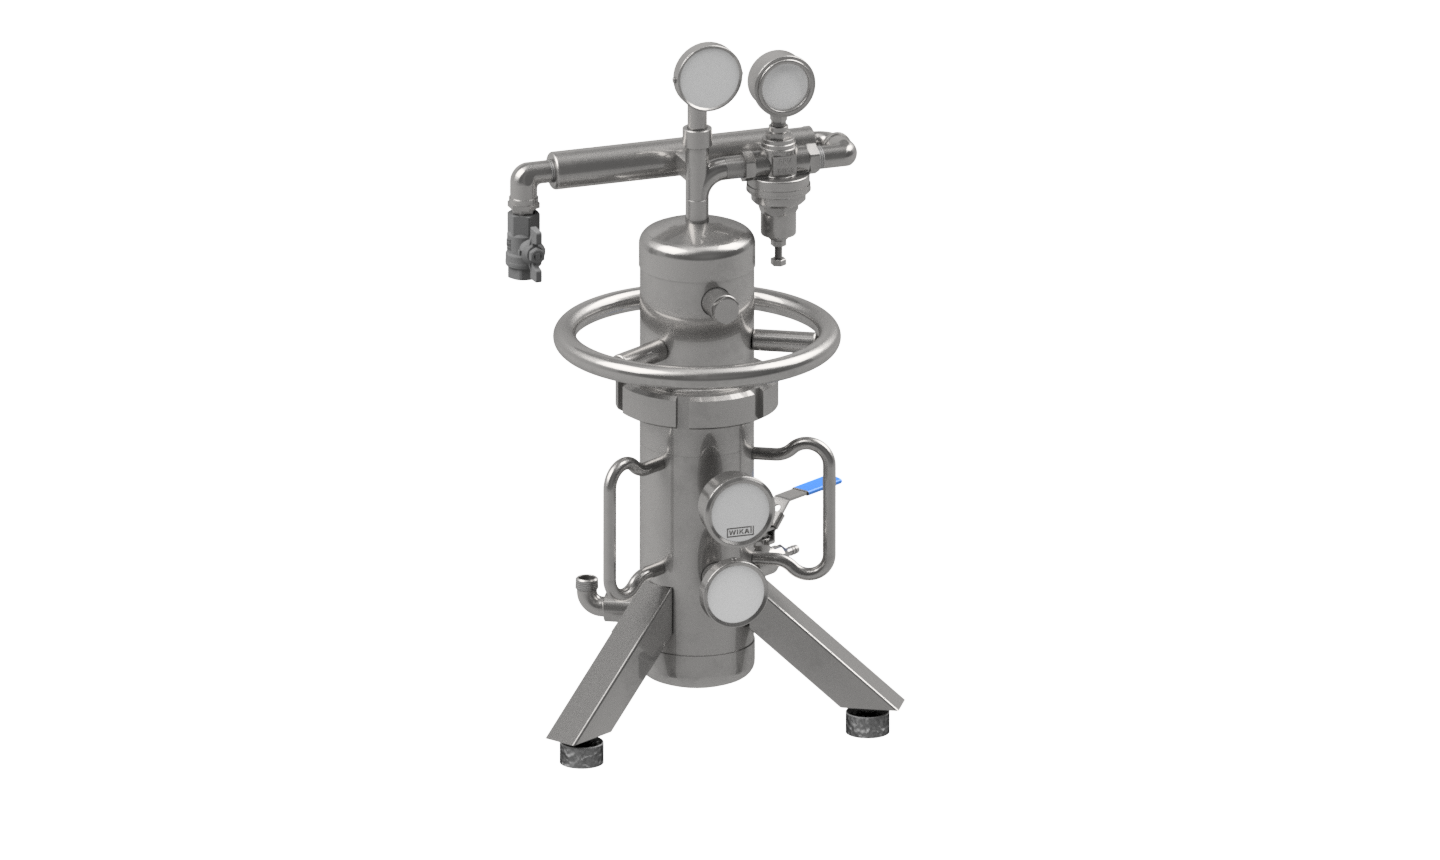
\includegraphics[keepaspectratio,width=\textwidth]{render.png}
    \caption{3D Darstellung des Dampfdruckbehälters}\label{fig:render}
\end{figure}

\par

Dies ist auch in Abbildung~\ref{fig:render} sehr gut zu erkennen (vgl. Abb.\ref{fig:render}).


\blindtext[2] \par


\section{Wahl der Dichtmittel}
\blindtext[2] \par

\section{Einflussgrößen auf die Auslegung nach AD2000}
\blindtext[1]


%Tabelle einfügen: 

\begin{table}[htb]
\centering
\begin{tabular}{|c|cc|} 
 \hline
 Einheit & Benennung & Kategorie \\ %[0.5ex] 
 \hline
 m & 6 & 8783 \\ 
 s & 7 & 78 \\
 V & 545 & 778\\
 A & 545 & 18744\\
 \hline
\end{tabular}
\caption{Eine sehr vielaussagende Tabelle}\label{vielaussagend}
\end{table}


Wie in Tabelle \ref{vielaussagend} zu erkennen, handelt es sich um eine sehr unwichtige Information, die hier gelistet ist.\blindtext[1]


\newpage
%\chapter{Kapitel mit einigen Formeln}
\blindtext{}


%Aufschreiben von Formeln:
%1. Möglichkeit: Equatation - Umfeld
% für eine Darstellung im Formelverzeichnis
% Caption: Beschriftung unter der Formel und im Verzeichnis
% Label: Referenz für Textverweise

\begin{formel}
\begin{equation}
   a=b\label{eq:Eq3}          %Label Referenz für Textverweise
\end{equation}
\caption{Grundformel 1}
\end{formel}

\begin{formel}
\begin{equation}
1+1=3\label{formel2}
\end{equation}
\caption{Schwerkraftsberechnung}
%\label{Berechnung der Schwerkraft}
\end{formel}


Mit diesen beiden Formeln ergeben sich verschiedene Möglichkeiten der Umformung, die für den weiteren Verlauf genutzt werden können:

%2. Möglichkeit: align Umgebung
%-> Vorteil: Intertext, Formatierung etc.

\begin{align}
a+b&=c
\intertext{Des Weiteren gilt:} 
b=c
\end{align}

Also was ist folglich c? Nach dem Tüv \cite[vgl.][S.~133]{VerbandderTUVe.V..2020} gilt:

\begin{formel}
\begin{equation}
    \label{eq:Eq10}
    Y=Kd \ast \left(Xd + \frac{1}{Tn} + \int Xd\ dt + d\ \frac{Xd}{dt}\right)
\end{equation}
\caption{Komplizierte Formel}
\end{formel}




\newpage
\chapter{Kapitel mit Symbolen und Zitaten}

Hier stehen gleich einige Symbole, die im Symbolverzeichnis aufgelistet werden sollen. Zu finden sind die Quellen auch im Literaturverzeichnis unter~\cite[S.~49]{Wittel.2021b}
\[\symE=\symm \symc^2\]

where \symE~is the energy \ldots
Die Formel entstammt der TüV eV \cite[S.~133]{VerbandderTUVe.V..2020}



\newpage
\chapter{Fazit und sicherheitstechnische Beurteilung der Facharbeit}
\blindtext{}
\par
\blindtext{}

% 
% weitere Dokumente / Kapitel
% 


% Schlussteil: 
\addtokomafont{chapterentry}{\vspace{-30pt}\rmfamily\mdseries\large \hspace{0pt}}
\newpage
\begin{appendix}

%PDF DIN A4 Seiten einbinden: Ort des Dokuments: Hauptordner
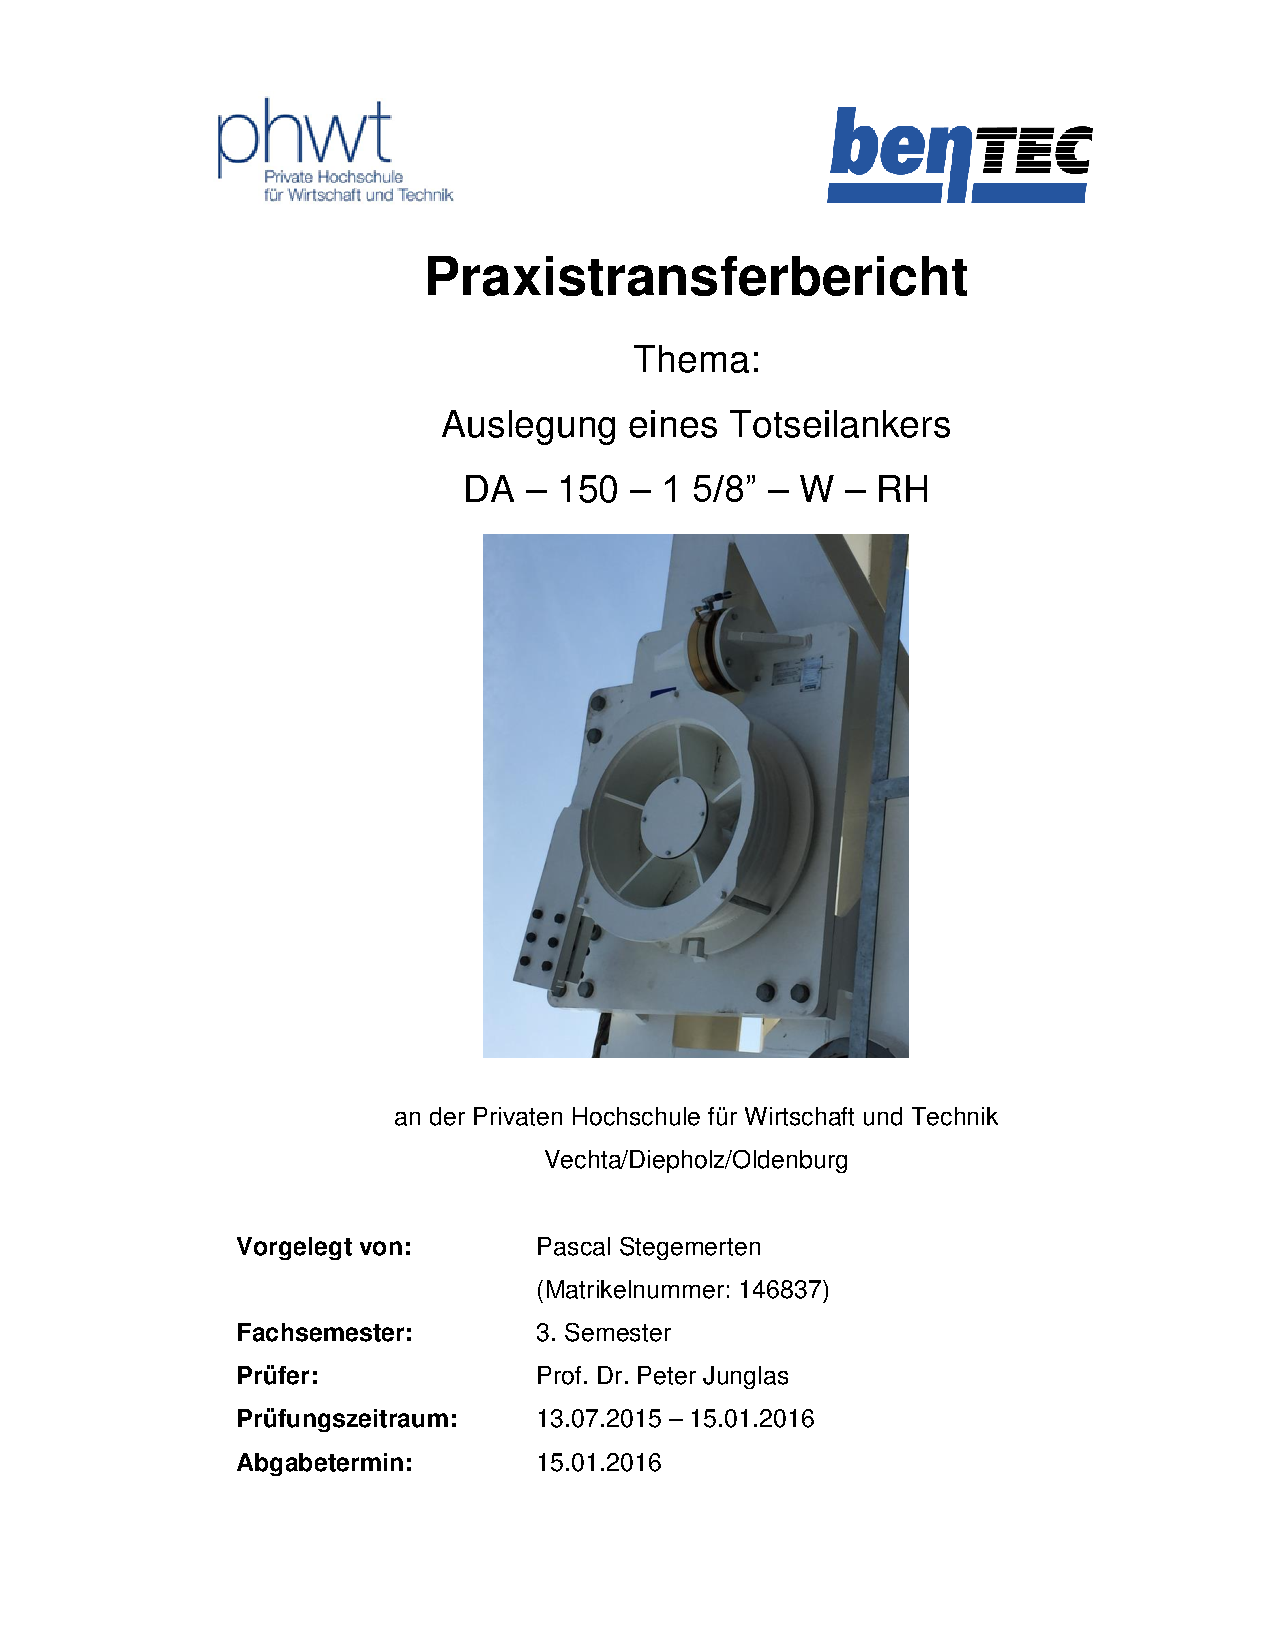
\includepdf[frame,pages=1,scale=0.9,pagecommand=\chapter{Auszug aus einem PTB}]{test3}
\includepdf[frame,offset=10mm 5mm,pages=2,scale=0.8,noautoscale=true,pagecommand=\chapter{Noch ein Auszug aus einem PTB}]{test5}


%DIN A3 pdf Seiten einbinden - benötigt noch weitere Anpassungen (Seitenzahl, Ränder, Geometrie)
%\KOMAoptions{paper=A3,paper=landscape, DIV=20}
%\newgeometry{left=4cm, right=2cm, top=2cm}
%\recalctypearea
%\addtokomafont{subsection}{\normalfont\large\rmfamily\mdseries\hspace*{3cm}\vspace{2cm}}
%\includepdf[fitpaper=true,frame,pages=1,scale=0.8,pagecommand=\chapter*{Anhang I: Zeichnung des Dampfablasses}]{test2}


%\KOMAoptions{paper=A4,pagesize, paper=portrait, DIV=20}
%\newgeometry{left=4cm, right=2cm, top=2cm}
%\recalctypearea
% offset=40mm 20mm zum Verschieben der pdf auf der Seite, pagecommand={\thispagestyle{empty}} für Seiten ohne seitenzahl

%delta=8mm 11mm, offset=5mm 7mm,
%trim=0 40mm 0 40mm, clip,  -> 

%Graphiken einfügen
\chapter{Auszug aus der Tabelle xy}
\begin{figure}[ht]
	\centering
  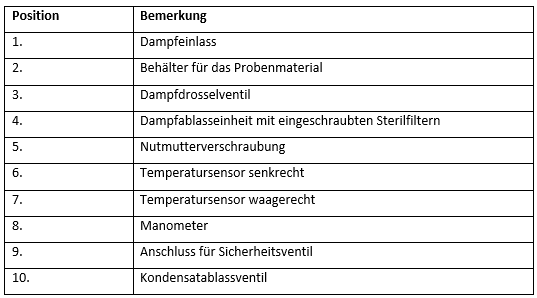
\includegraphics[width=\textwidth]{Anhang/tabelle1.png}
	%\caption{um 30 Grad gedreht}
	%\label{fig1}
\end{figure}





\end{appendix}
                     % Anhang
\newpage                                        
\printbibliography[title=Literaturverzeichnis]  % Literaturverzeichnis erstellen
\include{01_Konfig/1.5_erklärung}               % Eidestattliche Erklärung


\end{document}
